\subsection[]{Pixel- und Streifendetektoren}


\begin{frame}{Streifendetektoren}
	\begin{columns}[T]
		\column{.45\textwidth}
			\begin{figure}[htbp]
			  \centering
			   \includesvg[svgpath=bilder/, width=\textwidth]{streifen}
			  \caption*{$N^+/P^+$: hochdotiert}
			\end{figure}
	    \column{.5\textwidth}
	    	\begin{itemize}
			  \item Meist n-dotiertes Grundmaterial (Silikon) mit p-dotierten Streifen
			  \item einseitiger Streifendetektor $\rightarrow$ eindim. Ortsinformation
			  \item doppelseitig: Elektroden in nicht-parallele Streifen segmentieren (meist 90$^\circ$)
			  $\rightarrow$ zweidim. Ortsinformation
			\end{itemize}
    \end{columns}
\end{frame}

\begin{frame}{Pixeldetektoren}
	\begin{columns}[T]
		\column{.45\textwidth}
			\begin{figure}[htbp]
			  \centering
			  \includesvg[svgpath=bilder/, width=\textwidth]{pixel}
			  \caption*{$N^+/P^+$: hochdotiert}
			\end{figure}	
	    \column{.5\textwidth}
	    	\begin{itemize}
			  \item Elektroden in rechteckige Pixel segmentiert $\rightarrow$ zweidim. Ortsinformation
			  \item Pixelbreite ca 100$\mu$m
			  \item kleinere Elektrodenoberfläche besser um Signal zu verarbeiten (kleinerer Leckstrom)
			  \item hohe Kanalzahl
			\end{itemize}
    \end{columns}
\end{frame}


\begin{frame}{Pixeldetektoren}
			\begin{figure}[htbp]
			  \centering
			  \includesvg[svgpath=bilder/, width=\textwidth]{pixelstreifenvgl}
			  \caption*{Mehrfachtreffer in doppelseitigem Streifendetektor erzeugen Mehrdeutigkeiten bei
			  Zuordnung der Trefferkoordinaten}
			\end{figure}
			 \vspace{1cm}
\end{frame}


\begin{frame}{Pixel-/Streifendetektoren}
    \begin{columns}[T]
		\column{.45\textwidth}
			\textbf{Vorteile}		
			\begin{itemize}
			  \item gute Ortsauflösung $O(10\mu m)$  ($<$~MWPC/Driftkammer, aber Pixel~$<$~Streifen)
			  \item kleinere Energie, um $e^-$/Loch-Paar zu erzeugen $\rightarrow$ kleinere Variation der
			  Pulshöhe, höhere Energieauflösung
			  \item Pixeldetektoren erlauben einfache eindeutige Zuordnung
			\end{itemize}	
	    \column{.5\textwidth}
	    	\textbf{Nachteile}
	    	\begin{itemize}
			  \item teuer
			  \item hohe Verlustleistung (Kühlung notwendig)
			  \item begrenzte Haltbarkeit bei hoher Strahlung (nicht ionisierende Strahlung $\rightarrow$
			  z.B. Leerstellen im Gitter)
			  \item hohe Kanalzahl
			  \item Ausleseelektronik nah an aktiver Fläche
			\end{itemize}
    \end{columns}
   \end{frame}
   
\begin{frame}{Pixeldetektoren}
    \begin{columns}[T]
			\column{.5\textwidth}
				\begin{figure}[htbp]
				  \centering
				  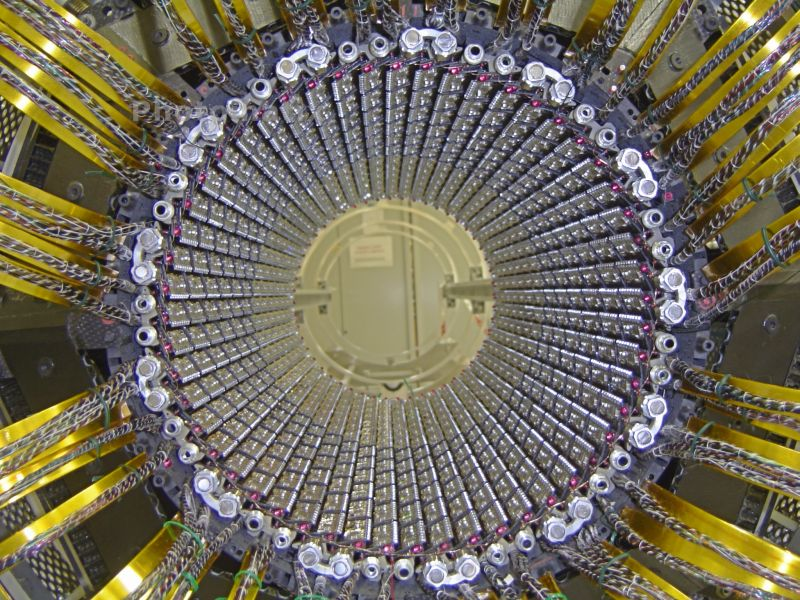
\includegraphics[width=\columnwidth]{bilder/beispiele/pixel_layer.jpg}
				\end{figure}
% 			 \vspace{1cm}

		 	 \column{.45\textwidth}		
		 	 \centering	 
				\begin{figure}[htbp]
				  \centering
				  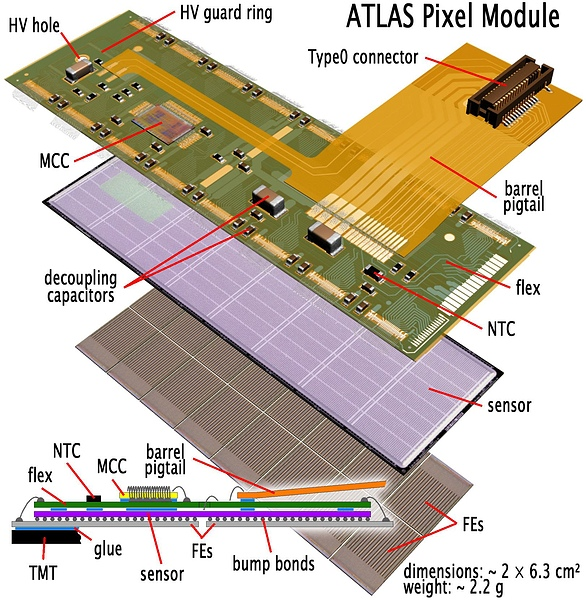
\includegraphics[width=0.9\columnwidth]{bilder/beispiele/module.jpg}
				\end{figure}
    \end{columns}
    \vspace{.6cm}
			ATLAS Pixel Detecor, LHC, CERN [pba]:\\
			Drei Lagen mit Radien 5, 9 und 12 cm;\\ 80 Millionen Pixel decken insgesamt 1,7~m$^2$ ab
\end{frame}
